\chapter{Overview of the existing System}
The internship project was not focused on creating an entirely new system from scratch, but rather on a deep redesign and restructuring of an existing system developed many years ago using legacy technologies and affected by several issues and critical limitations.

Before discussing the architectural, technological, and implementation choices that were made, it is necessary to carry out a thorough analysis of the current system, in order to understand its behavior, operational flows, technologies used, the main issues to be addressed, how to resolve them, how to prevent them from reoccurring in the future, and how to ensure that the new system is scalable and maintainable.

\section{System Design}

The \textit{SRP} system is fundamentally divided into two primary segments: 
\begin{itemize}
    \item Company Network;
    \item Client Network.
\end{itemize}

These segments interact and communicate exclusively through a \textit{DMI Console}, which acts as a unidirectional bridge, transferring requests from the client network to the internal company network. 

The overall architecture is depicted in the diagram in figure \ref{fig:as-is-system-design}.

\begin{figure}[h]
  \centering
  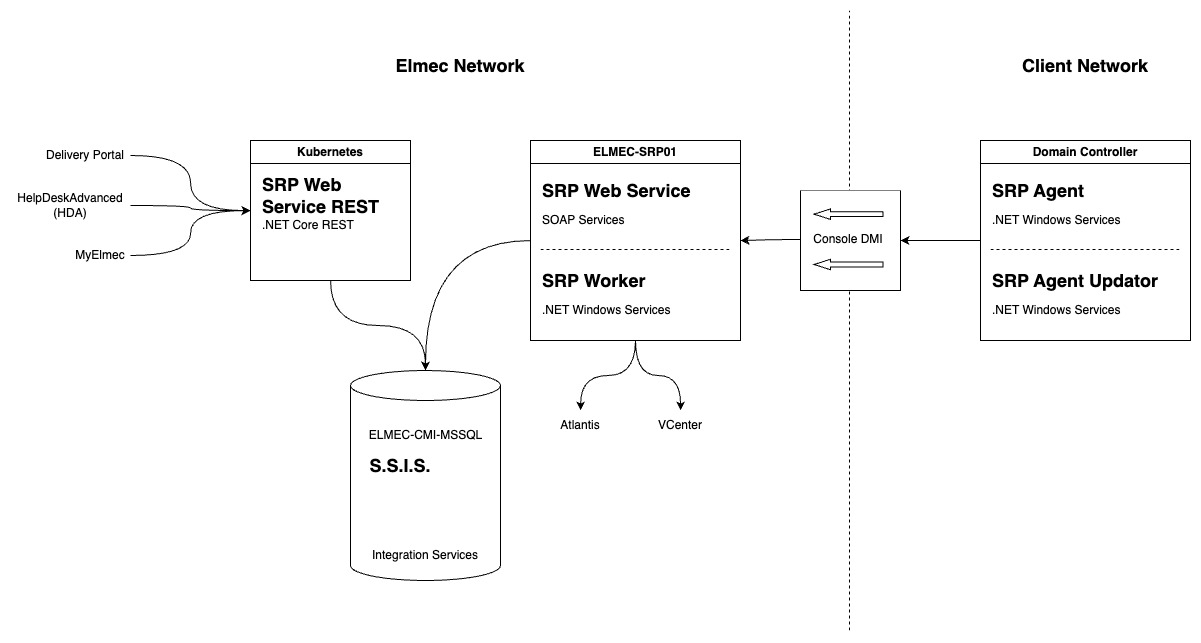
\includegraphics[width=1.0\textwidth]{images/as-is/SRP AS-IS (System Architecture).jpg}
  \caption{AS-IS System Architecture}
  \label{fig:as-is-system-design}
\end{figure}

The system's operational flow involves several key components across both networks, orchestrating the processing of service requests.

\subsection{Main Functionalities and Components}
The current \textit{SRP} system relies on a suite of interconnected components, each serving a specific role in the lifecycle of a service request.

Elmec Network Components:
\begin{itemize}
    \item \textbf{SRP Web Sevice REST}:  This component, deployed on a Kubernetes cluster, exposes .NET Core RESTful services. It serves as the primary interface for external systems such as:
    \begin{itemize}
        \item \textbf{Delivery Portal}: An asset management system used to manage Service Request catalog configuration and Elmec's internal and client servers;
        \item \textbf{HDA (HelpDeskAdvanced)}: A ticket management system. Each service request is intrinsically linked to an HDA ticket via an ID, and HDA is responsible for initiating and associating service requests with existing tickets.
        \item \textbf{MyElmec}: A client-facing portal enabling customers to create, manage, and monitor the various services provided by Elmec (e.g., servers, management software, cloud solutions).
    \end{itemize}
    The \textit{SRP Web Service REST} communicates with the \textit{ELMEC-CMI-MSSQL} server.
    \item \textbf{ELMEC-CMI-MSSQL}: This server hosts the central SQL Server Database for the SRP system. It is the persistent storage layer for all service request data and related information.
    \item \textbf{S.S.I.S. (SQL Server Integration Services)}: Running on the ELMEC-CMI-MSSQL server, SSIS packages are crucial for data transformation and import/export operations. They facilitate the transfer of data, such as master data (e.g., Active Directory users, Organizational Units, groups) sent by SRP Agents, into the database. Each SSIS package is designed to transform the received information for database insertion or vice versa.
    \item \textbf{ELMEC-SRP01}: This Windows Server functions as the core engine for service requests within the Elmec network. It houses all the PowerShell scripts associated with individual service requests, which are maintained by the Platform team. Key components residing on ELMEC-SRP01 include:
    \begin{itemize}
        \item \textbf{SRP WebServiceSoap}: This component provides SOAP services primarily for communication with the SRP Agent located on the client side. It interacts with the database to retrieve necessary information before exposing it to the agents for service request execution.
        \item \textbf{SRP InternalWorker}: A Windows service that operates similarly to the SRP Agent but executes entirely within the Elmec network. This is utilized for service requests that do not require interaction with the client's network or Active Directory (e.g., "no patch" service requests). The InternalWorker queries the database every 10 seconds for "internal worker" type jobs, connects to the SOAP service, retrieves the Service Request ID and its fields, and initiates job execution. It also monitors logs every 30 seconds to determine the job's status.
    \end{itemize}
\end{itemize}

The only component in the client's network is called \textbf{Domain Controller}, which represents the client's Active Directory domain controller, where the communication tools with Elmec are installed. It hosts:
\begin{itemize}
    \item \textbf{SRP Agent (.NET Windows Service)}: Typically, one agent is configured per client domain, specifically for Active Directory (AD) and Exchange-related service requests. This agent performs two main functions:
    \begin{itemize}
        \item Every 8 hours, it reads master data (AD users, OUs, groups) from the domain controller and sends it to ELMEC-SRP01 for storage via SSIS.
        \item Every 5 minutes, it queries ELMEC-SRP01 for pending Service Requests. Upon finding any, it requests detailed information, loads the corresponding PowerShell script, and executes it. After initiating the script, the agent informs ELMEC-SRP01 that the SR is "running" and proceeds to the next SR.
    \end{itemize}
    
    \item \textbf{SRP Agent Updator (.NET Windows Service)}: This service continuously monitors the SRP Agent folder for a file with a .new extension. If detected, it stops the SRP Agent, updates it, and restarts it
\end{itemize}

\subsection{Interactions and Communication between Customers and Company networks}
The Communication between the company network and the clients' networks is a critical aspect of the SRP system's operations and is handled through the \textbf{DMI Console}.

This interface acts as a secure bridge that transfers service requests from the client network to Elmec’s internal systems. The DMI Console does not allow outbound communication from Elmec to the client, ensuring a controlled and secure data flow. Requests originating from SRP Agents installed on the client's domain controllers are routed through this console, reaching the SRP01 server, which handles execution and status tracking internally.

\section{Service Requests Workflow}

The lifecycle of a Service Request within the current system is orchestrated through a series of defined states and automated processes, involving interactions between various components and human operators. The flow is designed to manage SRs from initiation to completion, handling approvals, execution, and potential errors.

In Figure \ref{fig:flowchart-as-is} a complete and detailed flowchart is shown that illustrates all flows and scenarios, including information on the jobs and components that manage the various sections of an SR's workflow.

\begin{figure}[htbp]
    \centering
    \includegraphics[width=\textwidth, height=\textheight, keepaspectratio]{images/as-is/Flowchart AS-IS.jpg}
    \caption{AS-IS Service Request Execution Workflow}
    \label{fig:flowchart-as-is}
\end{figure}

\subsection{SR Initiation and Initial State Management}
A Service Request can be initiated through two primary channels:

\begin{itemize}
    \item \textbf{Via MyElmec Portal}: Clients can submit an SR by completing a dedicated form from the MyElmec portal. Upon saving the form, a ticket is created in the HelpdeskAdvanced (HDA) system with a \texttt{QUALIFIED} status, and a corresponding Service Request is generated in SRP with a \texttt{NEW} status. These two entities are then linked via the HDA Ticket ID;
    \item \textbf{Via HDA Ticket by Elmec Operator}: Operators have the ability to associate a catalog SR directly with a ticket they are managing within the HDA interface. When the ticket is saved in a \texttt{DELEGATED} status, the SR is created in SRP with a \texttt{NEW} status, linked to the ticket, and immediately triggers the SR workflow within SRP.l
\end{itemize}

Following its creation, the system evaluates whether the Service Request requires approval by the operators. The logic for setting the initial SR and HDA ticket states is as follows:
\begin{itemize}
    \item \textbf{If approval is required}: the Service Request is set to \texttt{WAITING FOR APPROVAL} status, and the corresponding HDA ticket is set to \texttt{QUALIFIED}. A communication is added to the ticket, indicating that the SR needs validation from an operator before execution;
    \item \textbf{If no approval is required and it's linked to an automatism}: the Service Request enters a \texttt{PENDING} state, and the HDA ticket is set to \texttt{DELEGATED};
    \item \textbf{If no approval is required and it's not linked to an automatism}: the Service Request is \texttt{ASSIGNED}, and the HDA ticket is set to \texttt{PASSED}. A communication is added to the ticket, noting that the SR requires manual processing by an operator.
\end{itemize}

\subsection{Approval and Execution Workflows}
For SRs requiring approval (\texttt{WAITING FOR APPROVAL} state with an HDA \texttt{QUALIFIED} ticket), an operator's intervention is necessary to validate the request. The operator has three possible actions:
\begin{itemize}
    \item \textbf{Cancel the SR}: the HDA ticket is set to \texttt{CLOSED ABORTED}, the SR status becomes \texttt{DECLINED}, and a notification email is sent to the requesting client;
    \item \textbf{Request client modification}: the HDA ticket is set to \texttt{WAITING USER}, the SR status becomes \texttt{SUSPENDED}, and a notification email is sent to the client. The workflow pauses until the client modifies the SR via Elmec.com;
    \item \textbf{Approve the SR}: the HDA ticket is set to \texttt{DELEGATED}, and the SR status becomes \texttt{APPROVED}.
\end{itemize}

Once a SR is \texttt{APPROVED}, SRP manages its subsequent flow based on whether it is linked to an automatism:
\begin{itemize}
    \item \textbf{If the SR is linked to an automatism}: the SR transitions to a \texttt{PENDING} state, while the HDA ticket remains \texttt{DELEGATED}. This implies it's awaiting automated execution;
    \item \textbf{If the SR is not linked to an automatism}: the SR is immediately set to \texttt{ASSIGNED}, and the HDA ticket is moved to \texttt{PASSED}. A note is added to the ticket indicating that the SR requires manual processing.
\end{itemize}

An SR in \texttt{PENDING} state is awaiting the execution of its associated automatism. The outcome of this automated execution determines the next state:
\begin{itemize}
    \item \textbf{Successful execution}: the SR is set to \texttt{COMPLETED}, and the corresponding HDA ticket is set to \texttt{SOLVED};
    \item \textbf{Unsuccessful execution}: the SR transitions to an \texttt{ERROR} state, and the HDA ticket is set to \texttt{PASSED}. Communication regarding the error is added to the ticket for visibility within HDA.
\end{itemize}

The execution of Service Requests themselves can involve the SRP Agent on the client's Domain Controller for operations requiring client-side interaction (e.g., Active Directory or Exchange environment changes). The SRP Agent periodically checks \texttt{ELMEC-SRP01} for pending SRs. If found, it retrieves the SR details, loads the relevant PowerShell script, and executes it. The agent then informs ELMEC-SRP01 that the SR is running. Monitoring is performed by a scheduled READLOG task on the client side, which checks the PowerShell script's log file every minute. A "KEY" in the log indicates completion, prompting the SRP Agent to inform ELMEC-SRP01 to set the SR to COMPLETED, triggering an HDA status update. An "ERROR" key indicates failure, leading to the log being sent to ELMEC-SRP01 and an error signal. A timeout mechanism also signals an error if completion is not detected within a specified duration


\section{Problems and core issues of the current system}

%\begin{itemize}
%    \item Identification of existing challenges (dynamic forms, field management, etc.)
%    \item Impact of issues on managing SR
%    \item Examination of currently implemented solutions (e.g., use of Stored Procedures)
%\end{itemize}

L'analisi dell'architettura e del flusso di lavoro del sistema SRP nella sua forma attuale ha rivelato una serie di problematiche critiche che ne compromettono la scalabilità, la manutenibilità e l'affidabilità. Questi problemi sono profondamente radicati nelle scelte tecnologiche e di design fatte anni fa e si manifestano in diverse aree chiave del sistema, dalla gestione del catalogo all'esecuzione degli script e all'import delle anagrafiche da Active Directory.

\subsection{Architectural and Technological Challenges}

Il sistema SRP presenta una struttura architetturale frammentata e una complessa integrazione tra i suoi componenti principali, portando a diverse criticità.

\subsubsection{Monolithic Frontend Component}
L'interfaccia utente per la navigazione del catalogo delle Service Request e per la compilazione delle relative forms è un componente front-end Vue.js eccessivamente grande e complesso (quasi 11 mila righe). Questo rende le modifiche, le estensioni,  e le customizzazioni per clienti specifici estremamente difficili. La logica per la gestione di campi dinamici, le relazioni tra di essi, le regole di compilazione e la validazione dei campi sono tutte gestite a livello di frontend, mescolando logica di business e presentazione. 

Nello specifico, l'unica e sola informazione relativa ai campi che viene restituita dal servizio REST backend (SRPWebSeviceREST), oltre al nome del campo e alla sua mandatorietà, è il suo tipo. Diventa quindi facile immaginare come questa informazione, che dovrebbe essere solamente un'indicazione sul componente che dovrà essere renderizzato (e.g. textbox, select, radio button, etc..) diventa una sorta di identificatore di un qualcosa di più ampio, come ad esempio un campo con tipo e.g. \texttt{UPN} è un campo composto dal valore di un altro campo 'Display Name', concatenato a una \@, con suffisso il valore di una select le cui opzioni sono i domini del cliente, forniti da un servizio REST esterno.

\begin{itemize}
\item \textbf{Tight Coupling with DeliveryHub}: La gestione del catalogo, la definizione dei template di configurazione e il collegamento tra Service Request e script PowerShell sono interamente dipendenti da DeliveryHub. Questa dipendenza crea un "single point of failure" nella configurazione e limita la flessibilità, rendendo impossibile per Elmec creare operatività aggiuntive senza passare da questo sistema.
\item \textbf{Dependence on SRP Agent}: La gestione dell'Active Directory e delle risorse del cliente si basa su un SRP Agent installato direttamente sui Domain Controller. Questo approccio solleva diversi problemi:
\begin{itemize}
\item \textbf{Sicurezza e Permessi}: Spesso l'agente richiede credenziali con privilegi elevati (es. domain-admin), che i clienti sono sempre più restii a concedere.
\item \textbf{Affidabilità e Controllo}: Le configurazioni sull'agente e sul Domain Controller sono complesse e difficili da gestire centralmente, potendo causare errori di esecuzione e di sincronizzazione dei dati.
\item \textbf{Scalabilità}: La necessità di installare, configurare e manutenere un agente per ogni dominio cliente rappresenta un notevole onere operativo. Si stanno valutando alternative come sistemi di provisioning più moderni o l'integrazione con ORMIS per superare queste limitazioni.
\end{itemize}
\item \textbf{Obsolete Communication Patterns}: La comunicazione unidirezionale attraverso la \textit{DMI Console} crea un collo di bottiglia e complica la gestione delle operazioni asincrone. La comunicazione tra i componenti è spesso basata su polling (es. SRP Agent che interroga il server ogni 5 minuti), un approccio che introduce latenza e inefficienze.
\end{itemize}

\subsection{Code and Data Management Issues}

La gestione del codice e della persistenza dei dati è un altro aspetto critico del sistema, caratterizzato dalla mancanza di versionamento e di strumenti di debug moderni.

\begin{itemize}
\item \textbf{Unversioned and Undebuggable Stored Procedures}: L'utilizzo intensivo di Stored Procedures nel database ELMEC-CMI-MSSQL rappresenta uno dei maggiori punti di debolezza. Queste procedure contengono logica di business fondamentale e sono:
\begin{itemize}
\item \textbf{Non Versionate}: Non esiste un sistema di controllo versione centralizzato per le Stored Procedures. Le modifiche vengono apportate direttamente sul database, rendendo impossibile tracciare i cambiamenti, tornare a versioni precedenti o testare le modifiche in ambienti separati.
\item \textbf{Difficili da Debuggare}: Il debugging delle Stored Procedures è un processo complesso e macchinoso, richiedendo spesso l'accesso diretto e gli strumenti specifici del server SQL, con il rischio di influenzare l'ambiente di produzione.
\end{itemize}
\item \textbf{Inaccessible and Unversioned SSIS Jobs}: I pacchetti S.S.I.S. sono essenziali per l'importazione e l'esportazione dei dati (es. anagrafiche AD). Tuttavia, questi job risiedono fisicamente sul server ELMEC-CMI-MSSQL e l'unico modo per accedervi e modificarli è attraverso un desktop remoto. Questo approccio:
\begin{itemize}
\item Impedisce il versionamento e la collaborazione.
\item Limita l'accessibilità, rendendo la manutenzione e il debugging un'attività onerosa e rischiosa.
\item Crea un punto di fallimento centralizzato e un forte accoppiamento tra la logica di business di import/export e l'infrastruttura.
\end{itemize}
\item \textbf{Lack of Data Integrity and Consistency}: L'assenza di una tipizzazione dei campi chiara e la gestione delle relazioni a livello di frontend o attraverso logiche procedurali nel database possono portare a inconsistenze e errori. L'analisi del "template di configurazione" ha evidenziato l'uso di tipi di campi generici (Campo Libero, Campo Custom) e l'impostazione di regole di validazione nel frontend, senza una garanzia di coerenza a livello di backend.
\end{itemize}

\subsection{Maintenance and Operational Challenges}

La gestione quotidiana del sistema è resa complessa da diverse inefficienze e scelte obsolete:

\begin{itemize}
\item \textbf{Manual Creation of Catalog Items}: La creazione di nuovi campi nel catalogo richiede la creazione di una "finta" Service Request, un processo inefficiente e non standardizzato che evidenzia una lacuna nella gestione del catalogo stesso.
\item \textbf{Proliferation of Customer-Specific SRs}: La decisione storica di creare una Service Request separata per ogni cliente, anche per modifiche minori, ha portato a un catalogo con un numero molto elevato di SR. Questo approccio, sebbene concepito per prevenire la propagazione di errori, rende il catalogo ingombrante e difficile da navigare e manutenere.
\item \textbf{Ambiguity in SR Statuses}: L'interazione tra gli stati della Service Request e quelli del ticket HDA non è sempre chiara, con stati come PENDING o ASSIGNED che possono avere implicazioni simili o sovrapposte. La gestione dell'automazione è spesso nascosta dietro a logiche condizionali, rendendo difficile la comprensione del flusso di lavoro effettivo.
\end{itemize}

In conclusione, il sistema SRP nella sua forma attuale è afflitto da problemi di design, sicurezza, manutenibilità e scalabilità. La nuova architettura dovrà affrontare queste sfide introducendo un sistema più robusto, versionato e basato su principi di software design moderni.